\chapter{Sprint 0}

\section*{Introduction}
   Sprint 0 is an introductory chapter where we go over our hardware and software choices and we explain the Odoo architecture as well as the module structure

% Une section
\section{Hardware Environment}

Our application was developed using a portable computer and hosted on a Linux server.\\
\noindent Table 2.1 presents the developpment computer specifications: 
\begin{table}[H]
\centering
\caption{Computer Specifications}
\label{my-label}
\begin{tabular}{|p{.30\textwidth}|p{.60\textwidth}|}
\hline
\textbf{CPU} & I7-4600U\\
\hline
\textbf{RAM} & 8,0 GB   \\
\hline
\textbf{OS} & Microsoft Windows 10 x64 \\
\hline
\textbf{Storage} & 1 TB Hard Disk Drive \\
\hline

\end{tabular}
\end{table}






\section{Software environment and programming languages}
    % Une sous section

    % Une deuxième sous section
     \subsection*{Programming language}
         \begin{center}
         
\includegraphics[scale=0.8]{img/python102.png}\\
         \end{center}
    \textbf{Python} is an interpreted, high-level, general-purpose programming language. Created by Guido van Rossum and first released in 1991, Python's design philosophy emphasizes code readability with its notable use of significant whitespace..\cite{Python}\\
    We had to use Python as our programming language since its the only language Odoo supports\\
    Python is very popular, and that popularity came in handy when searching for documentation or libraries\\
     \subsection*{Markup Language}
         \begin{center}
         
\includegraphics[scale=0.9]{img/xml102.png}\\
         \end{center}
    \textbf{Extensible Markup Language (XML)} is a markup language that defines a set of rules for encoding documents in a format that is both human-readable and machine-readable.\cite{XML}\\
    We use XML to design our user interface according to the Odoo standards\\
    \subsection*{IDE}
         \begin{center}
         
\includegraphics[scale=0.8]{img/PyCharm102.png}\\
         \end{center}
    \textbf{PyCharm} is an integrated development environment (IDE) used in computer programming, specifically for the Python language. It is developed by the Czech company JetBrains. It provides code analysis, a graphical debugger, an integrated unit tester, integration with version control systems (VCSes).\cite{PyCharm}\\
    We opted for PyCharm because it offers various features including a python debugger\\
    We are using the "Community Edition", it is free and licensed under Apache2\\


  


    
    
    \subsection*{Database}

          \begin{center}
          
\includegraphics[scale=0.8]{img/Postgre102.png}\\
          \end{center}
    \textbf{PostgreSQL}, also known as \textbf{Postgre}, is a free and open-source relational database management system (RDBMS) emphasizing extensibility and SQL compliance. It was originally named POSTGRES, referring to its origins as a successor to the Ingres database developed at the University of California, Berkeley. In 1996, the project was renamed to PostgreSQL to reflect its support for SQL. After a review in 2007, the development team decided to keep the name PostgreSQL and the alias Postgres.\cite{Postgre}\\
    This choice is imposed by Odoo.\\
    The \textbf{pgAdmin} package is a free and open-source graphical user interface (GUI) administration tool for PostgreSQL.\\
    We use pgAdmin 3 for manual database manipulations
    

    
    \subsection*{CSVEditor}
  
          \begin{center}
          
\includegraphics[scale=0.8]{img/LibreOffice102.png}\\
          \end{center}
    \textbf{LibreOffice} is a free and open-source office suite, a project of The Document Foundation. It was forked in 2010 from OpenOffice.org, which was an open-sourced version of the earlier StarOffice. The LibreOffice suite consists of programs for word processing, creating and editing of spreadsheets, slideshows, diagrams and drawings, working with databases, and composing mathematical formulae\cite{LibreOffice}\\
    This editor is free and comes pre-installed in Ubuntu distributions. we use it to edit Odoo security files\\

    
    \subsection*{Modeling Tool}
          \begin{center}
          
\includegraphics[scale=0.8]{img/StarUML102.png}
          \end{center}
    \textbf{StarUML} is a sophisticated software modeler aimed to support agile and concise modeling.\\
    The key features of StarUML are:\\
    -Multi-platform support (MacOS, Windows and Linux)\\
    -UML 2.x standard compliant\cite{StarUML}
    
    
    
    
    
    
    
    
    
\section{Framework choice}
Choosing the correct ERP is a critical step in this project, it is a non-reversible choice so we had to make sure the framework we chose perfectly aligns with our project visions.\\
in the table below we compare three different ERPs based on multiple criteria.
       \begin{table}[H]
\caption{ Framework comparison }
\begin{tabular}{|p{3cm}|p{4,3cm}|p{4,3cm}|p{4,3cm}|}
\hline
\textbf{Framework}  &\textbf{Odoo}&\textbf{ERPNext}&\textbf{SAP Business One} \\
\hline
\textbf{Developper} & Odoo SA  & Frappé Technologies & SAP SE  \\
\hline
\textbf{Written in} &
Python, JavaScript and XML & Python and JavaScript & ABAP  \\
\hline
\textbf{Release} &
February 2005 & 2008 & April 2002  \\
\hline

\textbf{Utilisateurs} &
5 000 000 & 3 000 000 & 1 000 000  \\
\hline

\textbf{Système
d'exploitation} &
Linux, Unix, MacOS,
Windows &
Linux, MacOS  &
Linux, Windows
\\

\hline

\textbf{Licence} &
-GNU (Community)\newline{}-Proprietary
(Entreprise) & GNU GPLv3  & Proprietary\\
\hline
\textbf{DB support} & 
-PostgreSQL & -MariaDB & -SQL Server\newline{}-SAP HANA  \\
\hline
\textbf{Mobile support} &
Android and IOS & Android and IOS & Android and IOS\\
\hline
\textbf{Advantages} & 
\newline{}-Open Source\newline{}-Free\newline{}- 14,000+ third party modules\newline{}-Highly customizable
 & \newline{}-Open Source\newline{}-Free\newline{}-Easy-to-use interface
 & \newline{}-Secure\newline{}-Easy to setup\\
\hline


 \textbf{Disadvantages} & 
 \newline{}-Bad Documentation\newline{}-Some modules are proprietary
 & \newline{}-No Third Party modules\newline{}-Complexe
 & \newline{}-No Third Party modules\newline{}-High Cost\newline{}-Limited flexibility\\
\hline

\end{tabular}
\end{table}
        \begin{figure}[H]
         \begin{center}
         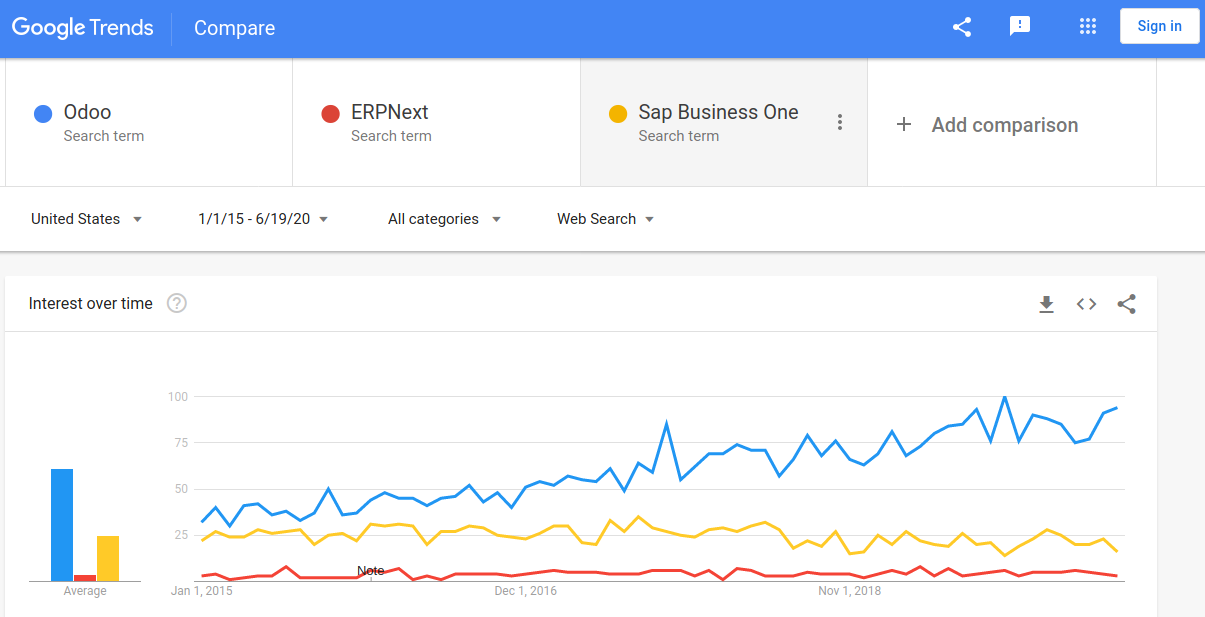
\includegraphics[scale=0.38]{img/framework-comparison.png}\\
         \caption{ERP popularity comparison}
         \end{center}
         \end{figure}


    
Odoo was the perfect ERP for the situation, offering great security and customizability, being free was also one of the deciding factors.
        
\section{Odoo ERP Structure}        
\subsection*{Odoo modules}
An application developed around Odoo or any other ERP, necessarily follows a modular architecture where each module covers a set of functionalities .\\
This type of architecture increases the flexibility of the application with respect to changing needs in the sense that it facilitates the extension of the application by adding other modules that are independent but communicate with the rest of the system.
\subsection*{Odoo Module structure}
       \begin{center}
         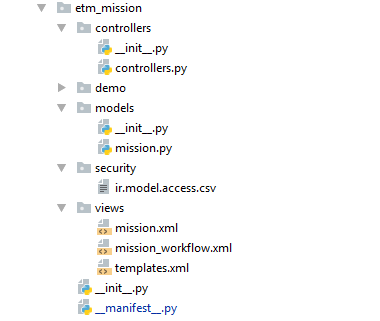
\includegraphics[scale=1]{img/project_Structure.png}\\
       \end{center}
       All files and folders concerning the module must be gathered in the same package with the name of the module.
     \begin{itemize}  
\item \textbf{\_\_init\_\_.py}: initialization file of the Python files in the directory
\item \textbf{manifest.py }: module description file

         \item\textbf{Models }: Directory containing all object classes and methods

         
\item\textbf{Views }: Directory containing all user interfaces and their actions as xml files\\
\item\textbf{Optional files }:
        \begin{itemize}
        \item\textbf{i18n }: Contains the translation of the module in different languages
        \item\textbf{Security }: Contains security rules to manage access rights for certain user groups to a model
        \item\textbf{Demo }: Contains data used to initialize the model's database table for demonstration purposes
         \end{itemize}
    \end{itemize}
    
    
\section{technical architecture}  
An Odoo system is formed from three main components:\\
the PostgreSQL \textbf{database server}, which contains all of the databases, each of which contains all data and most elements of the Odoo system configuration,\\
the Odoo \textbf{application server}, which contains all of the enterprise logic and ensures that Odoo runs optimally,\\
the \textbf{web server}, a separate application called the Open Object client-web, which enables you to connect to Odoo from standard web browsers.
       \begin{center}
         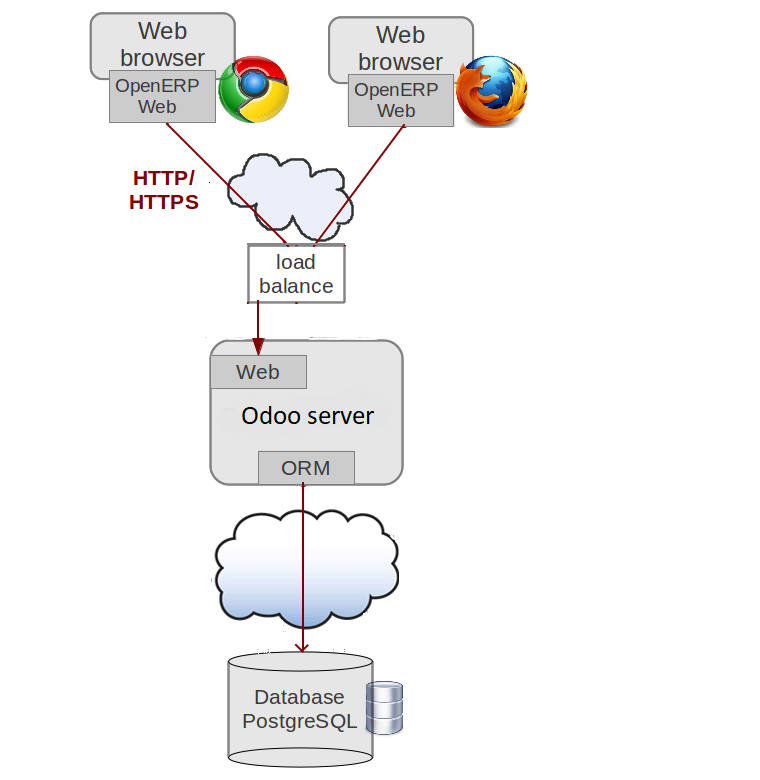
\includegraphics[scale=0.5]{img/terp_arch_1.png}\\
       \end{center}
\section{logical architecture}  
The following diagram shows the relationships between the different components of our project  

           \begin{center}
         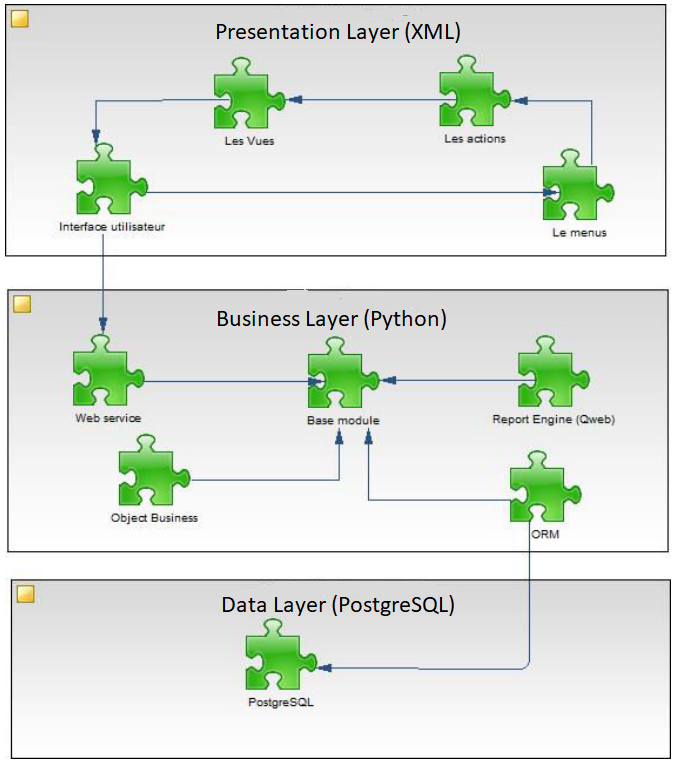
\includegraphics[scale=0.70]{img/logical_arch.png}\\
       \end{center}
\section*{Conclusion}
In this chapter, we studied the software and hardware environment and presented the architectural model of our framework Odoo. 
In the following, we will start the SPRINT1 which will be the subject of the first iteration of our project.